\chapter{Planning over Configuration Space Families}
\label{chap:family}

So far, we've been dealing with problems in a configuration space
with a fixed valid subset $\mathcal{C}_{\ms{free}}$.
In Chapter~\ref{chap:lazysp},
we described a lazy search algorithm which treats belief over edge
state in a binary fasion -- evaluated or unevaluated.
This deals with part of complexity.
Chapter~\ref{chap:utility} introduced the concept of utility to
motion planning,
and showed examples of its application to single-query motion
planning problems.
This deals with task efficiency, via utility functions.

However,
many applications exhibit structure beyond simple binary belief over
configuration validity.
In this chapter,
we introduce the \emph{family motion planning problem},
a generalization of the motion planning problem to a family of sets
over $\mathcal{C}$.
Since LEMUR accepts an arbitrary utility function.

Complex, but semi-structured.
Hint at beliefs over spaces.

In Section~\ref{sec:family:families-in-manipulation},
we motivate these problems in manipulation problems.

\section{Families in Manipulation Problems}
\label{sec:family:families-in-manipulation}

When addressing multi-step tasks
such as the table clearing task in
Figure~\ref{fig:family:herbarmmultithread-master},
the robot's valid subset $\mathcal{C}_{\ms{free}}$
changes each time an object is grasped or placed,
or when people or obstacles move.
Over the course of a planning episode,
these changing subsets constitute a family of related sets over
$\mathcal{C}$.

Here, I discuss motion and manipulation planning problems with
multiple moveable and graspable objects.
Discuss the composite configuration space.
Project everything down onto the robot's configuration space.

Use the workcell problem as an example.
Show images of each of the sets.
Forward-link to the experimental section later for full results.

This serves as a motivating example.
But the family motion planning problem is more general than this.

Motion planning approaches that build graphs
in the collision-free subset of
configuration space,
e.g. the
PRM \citep{kavrakietal1996prm}
and RRT \citep{lavallekuffner1999rrt},
have proven promising
for high-dimensional articulated robotics problems
in unstructured environments.
These approaches devote a large amount of computational effort
testing configurations and paths for collision,
and the resulting graph can then be reused
for other queries in the same collision-free subset.

However,
for manipuation problems,
this subset of the robot's configuration space
is sensitive to the locations and shapes of
both people and objects in the environment,
as well as the robot itself.
In addition, it depends on the shape and pose of any object
grasped by the robot.
This makes it difficult not only to apply the results of prior
planning computation to the current problem,
but also to efficiently consider planned or hypothesized motions,
since we must reconstruct our graph from scratch whenever
the environment changes.
This is especially the case for
multi-step manipulation tasks that must be planned into the future.
%We want to continuously update our representation for detours.

\subsection{Composite Space Projection}

Semi-structured environments between queries.

\begin{figure}
   \centering
   \begin{tikzpicture}
      \node at (0,0) {\includegraphics{build/family-composite/plot-volumes}};
      \node at (5,0) {\includegraphics{build/family-composite/plot-volumes-individual}};
   \end{tikzpicture}
   \caption{Volumes.}
\end{figure}

\begin{figure*}
   \centering
   \begin{tikzpicture}
      \node at (0,0) {\includegraphics{build/family-composite/plot-ptop-manifold}};
      \node at (5.5,0) {\includegraphics{build/family-composite/plot-g-manifold}};
      \node at (11,0) {\includegraphics{build/family-composite/plot-pbottom-manifold}};
   \end{tikzpicture}
   \caption{The trajectory projections.}
\end{figure*}


\subsection{Example Problems}

Manipulation problems.
Workcell example.
HERB exaple.

\subsection{Multiple Sets in a Family}

There will be more examples later in this chapter.

\subsection{Hints at a Solution}

For example,
consider the case where the robot has already evaluated a number
of roadmap edges in order to find a valid path to grasp the red mug.
Once grasped, the active valid subset $\mathcal{C}_{\ms{free}}$
has changed.
However,
any edge known to be valid for the previous step
can be validated in the new subset by simply checking the grasped
mug against the environment.

For more details, see Section~\ref{sec:family:approach} below.

See the forklift mega example problem
in Figure~\ref{fig:family:example}.

\begin{figure*}
   \begin{widepage}
   \begin{center}

   \subfloat[
      A two-part family problem in $\mathcal{C}$,
      first between $q_1$ and $q_2$ through $S_{12}$,
      then between $q_2$ and $q_3$ through $S_{23}$.
      The two free subsets $S_{12}$ and $S_{23}$ are distinct
      but related.
   ]{
      \includegraphics{build/figstar-a}
   }%
   \quad%
   \subfloat[
      The free subsets are related via other underlying
      subsets of $\mathcal{C}$, with $S_{12}=A \cap B$
      and $S_{23}=A \cap C$.
      A planner solving the first part (from $q_1$ to $q_2$)
      has found paths in $S_{12}$.
   ]{
      \label{subfig:family:figstar-intersections}
      \includegraphics{build/figstar-b}
   }%
   \quad%
   \subfloat[
      Due to the set relations,
      a planner solving the second part
      (from $q_2$ to $q_3$ in $S_{23}$)
      can reuse any segment known to be in $S_{12}$
      by checking only for its membership in $C$.
   ]{
      \includegraphics{build/figstar-c}
   }

   \vspace{0.1in}

   \subfloat[
      A forklift in a parking lot ($q_1$)
      must retrieve an object ($q_2$)
      and reverse park ($q_3$).
      This two-part problem
      requires plans in distinct collision-free
      $\mathcal{C}$-subsets
      $S_{12}$ and $S_{23}$.
   ]{%
      \begin{tabular}{c}
      \includegraphics{build/example-2d-a} \\
      \includegraphics{build/example-2d-b} \\
      \includegraphics{build/example-2d-c} \\
      \end{tabular}%
      \label{subfig:family:figstar-manip-probdef}
   }%
   \quad%
   \subfloat[
      Sets $S_{12}$ and $S_{23}$ are subsets of
      the configuration space of the robot $\mathcal{C}=\mbox{SE}(2)$,
      and can be represented as intersections
      of underlying subsets $A$, $B$, and $C$
      as in \protect\subref{subfig:family:figstar-intersections}.
   ]{%
      \label{subfig:family:figstar-manip-spaces}
      \begin{tabular}{c}
      \includegraphics{build/example-2d-d} \\
      \includegraphics{build/example-2d-e} \\
      \includegraphics{build/example-2d-f} \\
      \end{tabular}%
   }%
   \quad%
   \subfloat[
      After planning a path from $q_1$ to $q_2$ (top),
      a planner can reuse a configuration in $S_{12}$ (middle)
      by checking only for its membership in subset $C$,
      resulting in plan reuse (bottom).
   ]{%
      \begin{tabular}{c}
      \includegraphics{build/example-2d-g} \\
      \includegraphics{build/example-2d-h} \\
      \includegraphics{build/example-2d-i} \\
      \end{tabular}%
   }

   \caption[][99in]{x}
   \label{fig:family:example}

   \end{center}
   \end{widepage}
   
   \vspace{0.1in}
   \smallskip\noindent\small Figure \ref{fig:family:example}:
   An illustration of a family planning
   problem in a common configuration space $\mathcal{C}$.
   The problem definition generalizes to an artibrary number of
   configuration space subsets and set relations between them.
   When two queries in different subests are solved sequentially,
   a family planner can reuse path segments less expensively.
   See Section~\ref{sec:family:in-manipulation} for examples in
   manipulation.

\end{figure*}

Now that we see why it's useful to consider this decomposition,
let's formally define the problem.

\section{The Family Motion Planning Problem}
\label{sec:family:formulation}

The family planning problem is
a generalization of both the movers' problem
and the multi-query planning problem%
\cite{kavrakietal1996prm}.
The reader is referred to
Fig.~\ref{fig:family:example}
for a general example,
as well as a simple instantiation on a 2D manipulation task.
%which is discussed in more detail in
%Section~\ref{subsec:multi-prm-example}.
The family problem formulation
explicitly captures both planning and execution effort
and can therefore be used as an ensemble effort model
for use in the E$^8$-PRM planner across queries.

The family planning problem is multi-query in
a fixed configuration space $\mathcal{C}$.
However, unlike related problems in which all
queries demand solution paths contained within a single common subset of
$\mathcal{C}$
(usually the set of collision-free configurations, denoted
$\mathcal{C}_{\mbox{\scriptsize free}}$),
the family problem allows for the specification of
a \emph{family} of multiple such subsets
$\mathcal{F} = \{ A, B, \dots \}$.
Like $\mathcal{C}_{\mbox{\scriptsize free}}$,
each member of $\mathcal{F}$
is a subset of the common configuration space
(that is,
$S \subseteq \mathcal{C} \;\forall\; S \in \mathcal{F}$),
and each subset $S$ has its own indicator and planning estimator
${\bf 1}_S[\cdot]$ and $\hat{p}_S(\cdot)$
as in Section~??.
For example,
in Fig.~\ref{fig:family:example}\subref{subfig:family:figstar-manip-spaces},
$\mathcal{C}$-subset $B$
consists of configurations
free of collision between the robot and
the initial object pose.

The problem supports an arbitrary number of queries $\mathcal{U}$.
Each query $u$ demands a solution path through a \emph{single}
$\mathcal{C}$-subset $U \in \mathcal{F}$
(see Fig~\ref{fig:family:query-to-subset}):
\begin{equation}
  u : ( q_{start},\; q_{goal},\; U ) .
  \label{eqn:family:q}
\end{equation}

\begin{marginfigure}
   \centering
   \subfloat[Multi-query planning]{
      \includegraphics{build/query-to-subset-a}
   }
   \vspace{-0.05in}
   \subfloat[Family planning]{
      \includegraphics{build/query-to-subset-b}
   }
   \vspace{0.1in}
   \caption{While queries in multi-query planning reference
     the same subset of $\mathcal{C}$,
     each family query references one of a number of such sets.}
   \label{fig:family:query-to-subset}
\end{marginfigure}

\begin{marginfigure}
   \centering
   \subfloat[Containment relation]{
      \begin{tabular}{cc}
      \includegraphics{build/relations-inclusion} \\
      $A \subseteq B$ \\
      $\mathbf{1}_A \Rightarrow \mathbf{1}_B$ \\
      \end{tabular}
   }
   \vspace{-0.05in}
   \subfloat[Intersection relation]{
      \begin{tabular}{cc}
      \includegraphics{build/relations-intersection} \\
      $A = B \cap C$ \\
      $\mathbf{1}_B \wedge \mathbf{1}_C \Rightarrow \mathbf{1}_A$ \\
      \end{tabular}
   }
   \vspace{0.1in}
   \caption{Types of subset relations.
     Each relation can be expressed directly as set relations
     w.r.t a set $S$,
     or equivalently as logical statements
     on the corresponding indicator functions
     $\mathbf{1}_S(\cdot)$.}
   \label{fig:family:relations}
\end{marginfigure}

Finally, the family problem incudes a list of set relations
$\mathcal{R}$
between the $\mathcal{C}$-subsets in $\mathcal{F}$.
These can be expressed directly using set theoretic relations,
or equivalently as logical statements
on the corresponding indicator functions.
Common types of such relations
(containment and intersection)
are illustated in Fig.~\ref{fig:family:relations}.
Fig.~\ref{fig:family:example} gives an example of intersection relations;
an example of containment is a padded (conservative)
robot model (see Section~\ref{subsec:family:broad-phase}).

Together, these four elements
(a configuration space $\mathcal{C}$,
subsets $\mathcal{F}$ each with endowed indicators,
a set of queries $\mathcal{U}$,
and a list of subset relations $\mathcal{R}$)
comprise a family planning problem.

\subsection{Revisting the Example (as a Family Motion Planning Problem)}

Consider the diagram from Fig.~\ref{fig:family:example}.
$\mathcal{F}$ consists of five $\mathcal{C}$-subsets labeled
$A$, $B$, $C$, $S_{12}$, and $S_{23}$,
and we have two queries,
$u_{12}: (q_1, q_2, S_{12})$
and
$u_{23}: (q_2, q_3, S_{23})$.
$\mathcal{R}$ consists of the two relations
$S_{12} = A \cap B$ and $S_{23} = A \cap C$.
Suppose a cost model $\mathcal{M}$
wherein evaluating the indicator
$\mathbf{1}_A$ incurs cost 4,
evaluating $\mathbf{1}_B$ and $\mathbf{1}_C$ incurs cost 2,
and evaluating $\mathbf{1}_{S_{12}}$ and $\mathbf{1}_{S_{23}}$
incurs cost 6.
In the manipulation example in
Fig.~\ref{fig:family:example}\subref{subfig:family:figstar-manip-probdef},
this would be the case if each
pairwise outlined shape collision check incurs unit cost.

Suppose a graph structure within ${S_{12}}$ has been grown to solve
the first query $u_{12}$.
During the subsequent solve of query $u_{23}$,
an existing path segment known to be in ${S_{12}}$ can be shown to
also be contained within ${S_{23}}$ by only evaluating $\mathbf{1}_C$.
In the manipulation example,
reusing an a configuration from the previous search
would require only a check of cost 2,
instead of cost 6 for a new configuration.
Thus, we might hope that a planner may be biased towards reusing
said path segments in this case.

\subsection{Related Work}

Similarities to other problems.

It's a generalization.

Applicability of existing approaches.

Approaches which adapt a graph or tree structure
\citep{ferguson2006drrt, gayle2007lazyreconfigforest}
do not reason about this structure directly.

\cdnote{Is this the right place for this?}

\subsection{Review of Family Motion Planning Problems in Manipulation Tasks}

This briefly discusses how various types of problems can be viewed
as instances of the family motion planning problem.
Describe structure only, and forward reference to the applications
sections below.

Instances of family problems are especially prevalent when
planning for manipulation tasks with articulated robots.
This section details several such instances.
While these instances are discussed separately here,
they are often present simultaneously.
See Section~\ref{subsec:family:herb-experiment}
for experimental results for a problem
which includes several of the family problem instances
described below.

For multi-step plans, show the HERB bin example,
and the first few steps of the workcell example.

\subsection{Implementation Details}

We also provide an implementation for the
OpenRAVE \citep{diankov2010openrave}
virtual kinematic planning environment
which automatically discovers $\mathcal{C}$-subsets
in manipulation tasks.

\section{Approach: Reasoning over Family Beliefs}
\ref{sec:family:approach}

LEMUR relies on a domain-specific ensemble cost model
$\mathcal{M}$ to provide it with planning and execution cost
estimates for prospective edges.
This allows it to exploit this domain-specific structure.

We capture this structure via an ensemble cost model
$\mathcal{M}_{\ms{family}}$.
The model maintains
(a) a family $\mathcal{F}$ of $\mathcal{C}$-subsets
relevant to the problem,
(b) the inclusion/intersection relations between them,
and (c) the set of validity checks that have been performed
for each edge.
This knowledge enables it to implement an edge
planning cost estimator $\grave{p}_{\ms{family}}(e)$
which determines the minimum set of collision checks necessary
to validate an edge within a target subset.

\subsection{Family Belief States}

The problem is really about beliefs over states.
Talk about the family graph.
The belief space is $\mathcal{B}$,
so we're really planning over $\mathcal{B} \times \mathcal{C}$.

$\mathcal{C} \times \mathcal{B}$.

\subsection{Family Belief Graph}

\subsection{Set Relations as Logical Propositions.}
The planner represents the list of set relations $\mathcal{R}$
(Section~??)
specified in the family problem formulation
as a set of \emph{logical propositions} $P_{\ms{global}}$
which are considered globally applicable.
For example,
the proposition $\mathbf{1}_A \Rightarrow \mathbf{1}_B$
follows from the relation $A \subseteq B$
(see Fig.~\ref{fig:family:relations}).
In addition,
each edge $e$ in the roadmap $G$ is augmented with an initially empty
set $e.P$ containing all additional edge-specific propositions
known to be true as a result of any indicator functions evaluated
over that edge.
For example,
if planner evaluated the indicator $\mathbf{1}_B[e]$
and it returned False,
the proposition $\lnot\mathbf{1}_B$ would be added to $e.P$.
Together, such sets of propositions can be used as \emph{premises}
as part of an \emph{argument} to demonstrate a \emph{conclusion};
a logical solver can then be used validate or invalidate the argument.
For example, an argument with these premises and conclusion
$\{ (\mathbf{1}_A \Rightarrow \mathbf{1}_B), (\lnot\mathbf{1}_B) \}
\Rightarrow (\lnot\mathbf{1}_A)$
can be shown to be valid.

\subsection{A Utility Model}

The key to the Family PRM is the ensemble effort model
$\mathcal{M}_{\ms{multi}}$
(Algorithm~\ref{alg:family:effort-model})
which allows for evaluation of an edge
as well as estimates of its planning and execution effort
in a way that takes advantage of family structure.
The core of this model is the {\sc MultiOptCert} function
which takes as input an edge $q_e$,
a query $\mathcal{C}$-subset $U$,
and a set of known logical propositions $P_{\ms{known}}$
for that edge,
and as output produces an \emph{optimistic validation certificate}
consisting of subset indicators which if evaluated would
validate the membership of the edge in $U$ with lowest effort.

\begin{algorithm}
\caption{Family Validitiy Effort Model
   $\mathcal{M}_{\ms{multi}}$}
\label{alg:family:effort-model}
{\algrenewcommand\textproc{}% Used to be \textsc
\begin{algorithmic}[1]
\Function {$x_{\ms{multi}}$}{$e, U$}
   \State $(\mathcal{F}_{\ms{cert}}, b_{\ms{cert}}, {\hat p}_{\ms{cert}})
      \leftarrow \mbox{\sc MultiOptCert}(q_e, U,
      P_{\ms{global}} \cup e.P_{\ms{eval}})$
   \ForAll {$S \in \mathcal{F}_{\ms{cert}}$}
      \State $b_{\ms{eval}} \leftarrow \mathbf{1}_S[q_e]$
      \State $\arraycolsep=2pt
         e.P_{\ms{eval}} \leftarrow e.P_{\ms{eval}} \cup
         \left\{\begin{array}{rl}
         \mathbf{1}_S & \mbox{if } b_{\ms{eval}} \\
         \lnot \mathbf{1}_S & \mbox{otherwise} \\
         \end{array}
         \right\}$
      \If {$b_{\ms{eval}} \neq b_{\ms{cert}}(S)$}
         \State \Return $\infty$
      \EndIf
   \EndFor
   \State \Return $0$
\EndFunction
\Function {$\hat{x}_{\ms{multi}}$}{$e, U$}
   \State \Return $0$
\EndFunction
\Function {$\hat{p}_{\ms{multi}}$}{$e, U$}
   \State $(\mathcal{F}_{\ms{cert}}, b_{\ms{cert}}, {\hat p}_{\ms{cert}})
      \leftarrow \mbox{\sc MultiOptCert}(q_e, U,
      P_{\ms{global}} \cup e.P_{\ms{eval}})$
   \State \Return ${\hat p}_{\ms{cert}}$
\EndFunction
\end{algorithmic}
} %textproc
\end{algorithm}

\paragraph{Calculating the Family Optimistic Certificate}
%The \textsc{MultiOptCert} function (Alg.~\ref{alg:opt-edge-plan})
%performs the core reasoning which exploits the relations in
%the family problem.
The \textsc{MultiOptCert} function (Alg.~\ref{alg:family:opt-edge-plan})
is tasked with computing
the optimistically optimal set of indicator evaluations to perform
for the edge in order to validate its membership in the query
$\mathcal{C}$-subset $U$.
The function returns three elements:
(a) the family of $\mathcal{C}$-subsets
$\mathcal{F}_{\ms{cert}} \subseteq \mathcal{F}$
whose indicators are to be evaluated,
(b) a binary function $b_{\ms{res}}$
which provides the desired indicator result for each evaluation,
and (c) the total evaluation cost ${\hat p}_{\ms{cert}}$
given by the $\hat{p}_S[\cdot]$ functionals
(Section~\ref{sec:family:formulation}).

\begin{algorithm}
\caption{Family Optimistic Certification}
\label{alg:family:opt-edge-plan}
\begin{algorithmic}[1]
\Function {MultiOptCert}{$q_e, U, P_{\ms{known}}$}
   \State $\mathcal{T}_{\ms{imply}} \leftarrow \emptyset$
   \ForAll {$\mathcal{F}_{\ms{cert}} \in \mathcal{P}(\mathcal{F})$}
         \label{line:family:power-set}
      \State ${\hat p}_{\ms{cert}} \leftarrow \sum_{S \in \mathcal{F}_{\ms{cert}}} \hat{p}_S[q_e]$
      \ForAll {$b_{\ms{res}} \mbox{ \textbf{s.t.} }
            b_{\ms{res}} : \mathcal{F}_{\ms{cert}} \rightarrow \{\mbox{True},\mbox{False}\}$}
            \label{line:family:all-binary-functions}
         \State $\arraycolsep=2pt
            P_{\ms{res}} \leftarrow
            \left\{\left. \begin{array}{rl}
            \mathbf{1}_S & \mbox{if } b_{\ms{res}}(S) \\
            \lnot \mathbf{1}_S & \mbox{otherwise} \\
            \end{array}
            \right|
            S \in \mathcal{F}_{\ms{cert}}
            \right\}$
         \If {$P_{\ms{known}} \cup P_{\ms{res}}
               \Rightarrow \mathbf{1}_U$ is valid}
            \State $\mathcal{T}_{\ms{imply}} \leftarrow
               \mathcal{T}_{\ms{imply}} \cup
               \{ (\mathcal{F}_{\ms{cert}}, b_{\ms{res}}, {\hat p}_{\ms{cert}}) \}$
         \EndIf
      \EndFor
   \EndFor
   \State \Return $(\mathcal{F}_{\ms{cert}}, b_{\ms{res}}, {\hat p}_{\ms{cert}})
      \in \mathcal{T}_{\ms{imply}}$
      with lowest ${\hat p}_{\ms{cert}}$
\EndFunction
\end{algorithmic}
\end{algorithm}

The function accumulates a set $\mathcal{T}_{\ms{imply}}$ of
valid certificates which would imply membership in $U$.
We proceed by considering all combinations of
available $\mathcal{C}$-subset indicators
$\mathcal{F}_{\ms{cert}}$ (line~\ref{line:family:power-set}).
For each set of evaluations,
we compute the planning effort ${\hat p}_{\ms{cert}}$
which would be required.
We then consider all possible outcomes for each indicator
by iterating over all functions $b_{\ms{res}}$ mapping
from $\mathcal{C}$-subset $S$ to binary values
(line~\ref{line:family:all-binary-functions}).
For each potential outcome $b_{\ms{res}}$,
we form the set of additional propositions $P_{\ms{res}}$,
and then use a propositional logic solver to determine whether
the aggregate premises imply membership
in the query $\mathcal{C}$-subset $U$.
If so, this certificate is added to $\mathcal{T}_{\ms{imply}}$,
and the lowest-effort certificate is returned.

\section{Family Belief as a Utility Model}

We show preliminary results of applying LEMUR to planning over
such $\mathcal{C}$-space families on the sequential
three-step task in
Figure~\ref{fig:family:herbarmmultithread-master}.
Such a planner can be seen as a generalization of self-collision checked
\citep{leven2002changing} or dynamic \citep{jaillet2004dynamicprm}
roadmaps to a larger number of subsets.

This section lays out how to leverage the family formulation
as a planning effort model
for use in the E$^8$-PRM.
The resulting algorithm,
the Family PRM,
exploits the family structure inherent in manipulation problems
by efficiently reuses planning computation between related queries.

The Family PRM (Algorithm~\ref{alg:family:prm}) is a simple
extension of the \mbox{E$^8$-PRM}
(Section~??).
They key differences are that
(a) it reasons about $\mathcal{C}$-subsets
using logical propositions,
and (b) it uses a family ensemble effort model
$\mathcal{M}_{\ms{family}}$ to capture relations
between these subsets.

\subsection{Relation to Previous Work}

A large body of prior work has focused on methods to
improve planning efficiency on manipulation problems.
We show that many of these approaches are
in fact special instances of a more general structure,
which we formulate as the \emph{family planning problem}.

\subsection{Show some examples of the behavior?}

\section{Application: Caching Invariant Geometry}

\paragraph{Cached Self-Collision-Checked Roadmaps}
\label{subsec:family:cached-self-valid}

Self-collision checking is a potentially expensive component to
articulated motion planning;
in contrast to environment checking,
it is fundamentally quadratic in the number of moving links.
Further, pairs of links to be checked
tend to be relatively close to each other,
reducing the effeciveness of broad-phase approaches.

Leven and Hutchinson \citep{leven2000changing}
introduced the concept of a pre-cached roadmap consisting of
configurations and paths already known to be valid w.r.t.
self-collision.
As a type of invariant in $\mathcal{C}$,
this can be seen as a particular instance of family planning.
See Fig.~\ref{fig:family:self-collision-example}.

\begin{figure*}
   \centering   
   \includegraphics{build/family-sq-caching/pvxs}
   \caption[]{LEMUR single-query results on several HERB problems,
      all using baked calls.
      Traces are LEMUR
      (\protect\tikz{\protect\draw[thick,black] (0,0) -- (0.15,0.15);}),
      the family planner (no caching)
      (\protect\tikz{\protect\draw[thick,blue] (0,0) -- (0.15,0.15);}),
      or the family planner with self-checked caching
      (\protect\tikz{\protect\draw[thick,green] (0,0) -- (0.15,0.15);}).}
\end{figure*}

\section{Application: Multi-Step Manipulation Tasks}

\paragraph{Grasped Objects}
\label{subsec:family:grasped-objects}

One instance specific to manipulation problems is the handling of
grasped objects.
For example, 
consider a manipulator which grasps a geometric object.
This affects the set of collision-free configurations
across a large section of $\mathcal{C}$
relative to the old set of valid configurations $S_{\ms{old}}$.
However,
the resulting $\mathcal{C}$-subset $S_{new}$
can be represented simply as
$S_{\ms{new}} = S_{\ms{old}} \cap G$,
with $G$ the set of robot configurations in which
the \emph{grasped object} (only)
is deemed free of collision with the robot and environment.
This structure is discussed in the context of the
\emph{conditional reachability graph},
part of the \textsc{FFRob} heuristic framework
\citep{garrett2014ffrob}.

For example,
consider the manipulation problem in
Figure~\ref{fig:family:testherb-problem}.
The robot must find a path which moves its arm to grasp the cup.
After the cup is grasped,
the robot can reuse any edge in the existing roadmap
by simply checking the grasped cup
against the remainder of the environment.
This structure,
together with the approach to dynamic environments,
are included together in the experimental results
(Section~\ref{subsec:family:herb-experiment}).

\begin{marginfigure}
   \centering
   \includegraphics{build/self-collision}
   \caption{A roadmap is pre-computed in $R$,
      the subset of $\mathcal{C}$ consisting of configurations free
      of robot self-collision.
      Online, the planner must find a path that's also within $E$,
      the subset free of environment collision.
      When solving this query in $S = R \cap E$,
      the Family PRM automatically prefers potential paths with
      pre-computed edges (e.g. shown in grey)
      due to lower planning costs over alternatives with lower
      execution costs.}
   \label{fig:family:self-collision-example}
\end{marginfigure}

\subsection{Prescribed Steps}

We tested the Family PRM on the manipulation task
described in Fig.~\ref{fig:family:testherb-problem}.
We used the $r$-disk PRM construction rule with $r=2.0$ rad,
and a batch size of $N=1000$.
Planning times are measured on a Lenovo T430s laptop.
The planner was asked to solve each of the steps of the plan
sequentially.

We varied
(a) the planning vs. execution parameter $\lambda$
(see Chapter~\ref{chap:utility}), and
(b) the subset relations provided to the planner
as described in Section~\ref{subsec:family:dynamic-environments}.
We measured the time required for planning (s)
and the length of the resulting solution resulting path (rad)
for each step of the task.

Note that the Family PRM,
with no relations specified and $\lambda=0$
reduces to the Lazy PRM.
As expected,
increasing $\lambda$ resulted in decreased planning times
but yielded longer paths.
Including more $\mathcal{C}$-subset relations
also significantly reduced planning times,
and had little effect on path lengths on this problem.
Note that the planning time results when using
the cached self-collision-checked roadmap, denoted by (*),
do not include the pre-computation time.

Note that including inter-step relations drastically
reduces planning times for subsequent steps.
We expect this trend would continue as more steps are included.
Also, note that when $\lambda=0$,
path length is unchanged as the number of set relations is
changed
-- this is because the paths that are selected for evaluation
by the algorithm are a function only of their (constant) lengths.

\begin{figure}
   \centering
   \includegraphics{build/workcell/configs}
   \caption{Robot tending a press brake in an industrial workcell.
      This example problem is reproduced from the Lazy PRM paper
      \citep{bohlin2000lazyprm}.
      The multi-step manipulation task requires eight motion planning
      problems in seven different $\mathcal{C}$-subsets.
      From its initial configuration (A),
      the robot moves to grasp a raw sheet (B)
      and transfer first to a settling table (C)
      and subsequently to the press brake (D).
      After the first bend, the robot receives the partially worked
      part (E) and uses a regrasping fixture (F)
      to regrasp it on the other side (G).
      After its second bend (H) and (I),
      the finished part is moved to the final pallet (J)
      before the robot returns to its initial configuration (A).
      Results for planning these steps are shown in
      Figure~\ref{fig:family:workcell-pvx}.}
\end{figure}

\begin{figure}
   \centering
   \includegraphics{build/multistep-prescribed/workcell}
   \caption[]{Example of planning over families for an industrial
      workcell example problem.
      Individual LEMUR results are dashed
      (\protect\tikz{\protect\draw[thick,densely dotted] (0,0) -- (0.15,0.15);}),
      while Family-aware results are solid
      (\protect\tikz{\protect\draw[thick,solid] (0,0) -- (0.15,0.15);}),.
      Colors for the inner search algorithm are:
      \protect\tikz{\protect\node[fill=red,draw=black]{};}\;RRT,
      \protect\tikz{\protect\node[fill=blue,draw=black]{};}\;IncBi,
      \protect\tikz{\protect\node[fill=olive,draw=black]{};}\;A*, and
      \protect\tikz{\protect\node[fill=cyan,draw=black]{};}\;LPA*.
      These results use $R\approx2.17$ scaled by $\log(n)/n$.}
   \label{fig:family:workcell-pvx}
\end{figure}

\begin{figure}
   \centering
   \includegraphics{build/multistep-prescribed/workcell-r1p3128ll}
   \caption[]{OLD VERSION.
      Example of planning over families for an industrial
      workcell example problem.
      Individual LEMUR results are dashed
      (\protect\tikz{\protect\draw[thick,densely dotted] (0,0) -- (0.15,0.15);}),
      while Family-aware results are solid
      (\protect\tikz{\protect\draw[thick,solid] (0,0) -- (0.15,0.15);}),.
      Colors for the inner search algorithm are:
      \protect\tikz{\protect\node[fill=red,draw=black]{};}\;RRT,
      \protect\tikz{\protect\node[fill=blue,draw=black]{};}\;IncBi,
      \protect\tikz{\protect\node[fill=olive,draw=black]{};}\;A*, and
      \protect\tikz{\protect\node[fill=cyan,draw=black]{};}\;LPA*.
      These results use $R=2.5$ scaled by $\log(\log(n))/n$.}
   \label{fig:family:workcell-pvx}
\end{figure}

\begin{figure*}[t]
   \centering
   
   \subfloat[Starting Configuration]{
      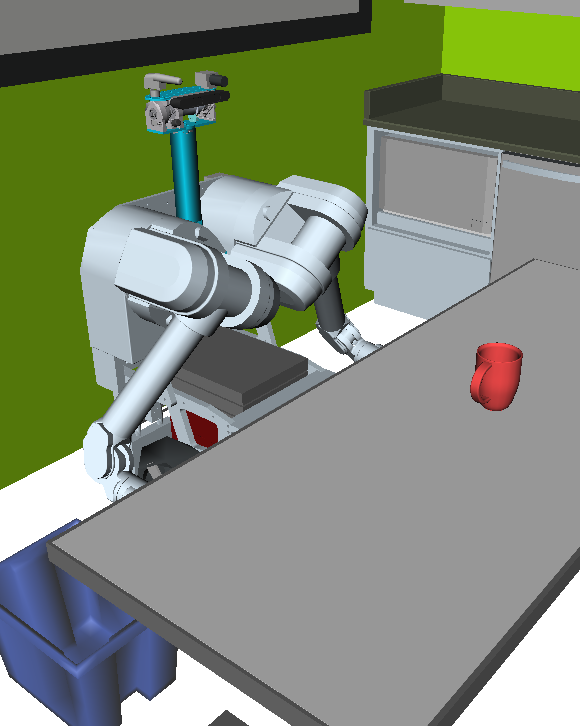
\includegraphics[width=0.185\linewidth]{figs/testherb-a.png}
   }
   \subfloat[Step 1, in $S_1$]{
      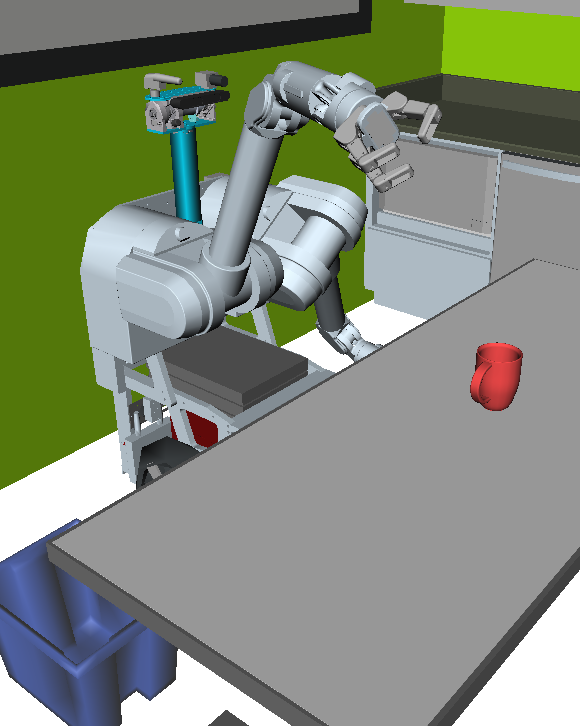
\includegraphics[width=0.185\linewidth]{figs/testherb-b.png}
   }
   \subfloat[Step 2, in $S_2$]{
      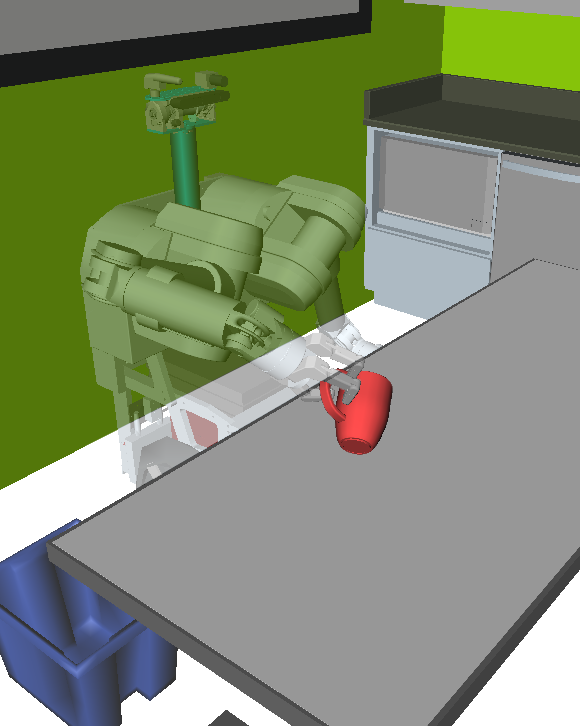
\includegraphics[width=0.185\linewidth]{figs/testherb-c.png}
   }
   \subfloat[Step 3, in $S_3$]{
      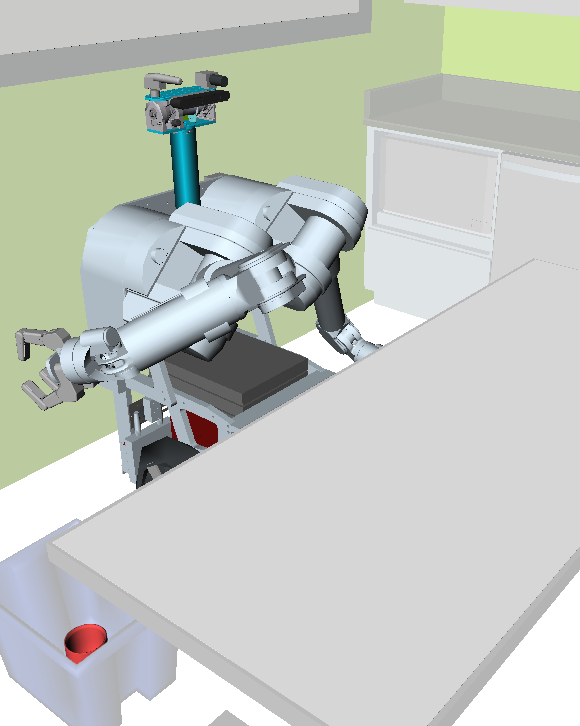
\includegraphics[width=0.185\linewidth]{figs/testherb-d.png}
   }
   \subfloat[Ending Configuration.]{
      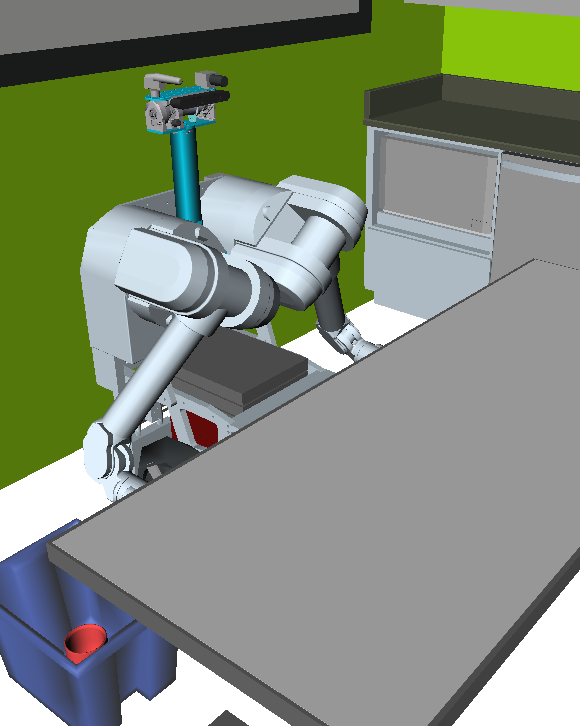
\includegraphics[width=0.185\linewidth]{figs/testherb-e.png}
   }

   \caption[][0.2in]{
     A home robot performing a three-step manipulation task.
     It must move from its home configuration
     to grasp the cup,
     transfer it to a drop location above the bin,
     and return home.
     Experimental results for the Family PRM
     are shown in Table~\ref{tab:family:testherb}}
   \label{fig:family:testherb-problem}
\end{figure*}

\begin{figure}
   \centering
   \includegraphics{build/multistep-prescribed/herbbin}
   \caption{Example of planning over families for the HERB bin example
      problem.
      Individual LEMUR results are dashed
      (\protect\tikz{\protect\draw[thick,densely dotted] (0,0) -- (0.15,0.15);}),
      while Family-aware results are solid
      (\protect\tikz{\protect\draw[thick,solid] (0,0) -- (0.15,0.15);}),.
      Colors for the inner search algorithm are:
      \protect\tikz{\protect\node[fill=red,draw=black]{};}\;RRT,
      \protect\tikz{\protect\node[fill=teal,draw=black]{};}\;IncBi-Old,
      \protect\tikz{\protect\node[fill=blue,draw=black]{};}\;IncBi,
      \protect\tikz{\protect\node[fill=olive,draw=black]{};}\;A*, and
      \protect\tikz{\protect\node[fill=cyan,draw=black]{};}\;LPA*.
      The IncBi-Old results used $R=2.0$ scaled by $1/n$.
      The new results use $R\approx2.54$ scaled by $\log(n)/n$.
      }
\end{figure}

\begin{table*}[b]
   \begin{widepage}
   \centering
   \footnotesize
   \setlength{\tabcolsep}{3pt}
   \renewcommand{\arraystretch}{1.3}
   \begin{tabular}{|cc|r@{ }lr@{ }lr@{ }lr@{ }l|r@{ }lr@{ }lr@{ }lr@{ }l|r@{ }lr@{ }lr@{ }lr@{ }l|}
   \toprule
   \multirow{2}{*}{Relations} & \multirow{2}{*}{Cost}
     & \multicolumn{8}{c|}{$\lambda = 0$}
     & \multicolumn{8}{c|}{$\lambda = 0.5$}
     & \multicolumn{8}{c|}{$\lambda = 1$}
   \\
     &
     & Step & 1 & Step & 2 & Step & 3 & \multicolumn{2}{c|}{Total}
     & Step & 1 & Step & 2 & Step & 3 & \multicolumn{2}{c|}{Total}
     & Step & 1 & Step & 2 & Step & 3 & \multicolumn{2}{c|}{Total}
   \\ \midrule
   \multirow{2}{*}{None} & Plan
     &  6.16&s &  3.72&s &  2.38&s & 12.25&s
     &  5.52&s &  2.89&s &  2.12&s & 10.53&s
     &  3.39&s &  2.25&s &  2.12&s &  7.76&s
   \\
     & Exec
     & 14.22&rad &  8.51&rad &  4.23&rad & 26.97&rad
     & 15.07&rad & 10.60&rad &  4.23&rad & 29.89&rad
     & 15.07&rad & 10.60&rad &  4.23&rad & 29.89&rad
   \\ [1ex]
   Inter-Step & Plan
     &  6.40&s &  2.33&s &  0.86&s &  9.59&s
     &  5.40&s &  1.55&s &  0.91&s &  7.86&s
     &  3.38&s &  0.91&s &  0.30&s &  4.59&s
   \\
   (Sec.~\ref{subsec:family:dynamic-environments},~\ref{subsec:family:grasped-objects})
     & Exec
     & 14.22&rad &  8.51&rad &  4.23&rad & 26.97&rad
     & 15.07&rad & 12.21&rad &  4.23&rad & 31.51&rad
     & 15.07&rad & 12.21&rad &  7.11&rad & 34.40&rad
   \\ [1ex]
   Self-Checked & Plan*
     &  3.54&s &  2.23&s &  1.17&s & 6.94&s
     &  2.99&s &  1.77&s &  1.16&s & 5.92&s
     &  1.47&s &  1.22&s &  1.16&s & 3.85&s
   \\
   (Sec.~\ref{subsec:family:cached-self-valid}) & Exec
     & 14.22&rad &  8.51&rad &  4.23&rad & 26.96&rad
     & 14.22&rad & 10.06&rad &  4.23&rad & 28.51&rad
     & 14.22&rad & 10.60&rad &  4.23&rad & 29.05&rad
   \\ [1ex]
   \multirow{2}{*}{Both} & Plan*
     &  3.25&s &  1.79&s &  0.90&s & 5.94&s
     &  2.88&s &  1.55&s &  0.92&s & 5.35&s
     &  1.47&s &  1.88&s &  0.31&s & 3.66&s
   \\
     & Exec
     & 14.22&rad &  8.51&rad &  4.23&rad & 26.96&rad
     & 14.22&rad &  8.51&rad &  4.23&rad & 26.96&rad
     & 14.22&rad &  9.64&rad &  6.36&rad & 30.22&rad
   \\ 
   \bottomrule
   \end{tabular}
   \caption[][-0.1in]{Home robot manipulation task results.
     The entry with no relations and $\lambda=0$ is equivalent
     to the LazyPRM.
     These are old results.}
   \label{tab:family:testherb}
   \end{widepage}
\end{table*}

\begin{figure}
   \centering
   \hspace{0.2cm}
   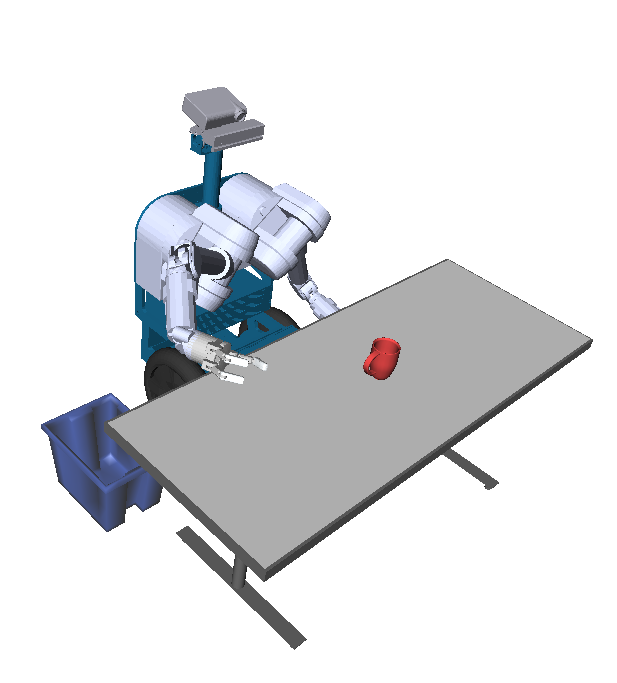
\includegraphics[width=2.7cm]{figs/herbarmmultithread/herbarmmultithread-step0.png}%
   \;
   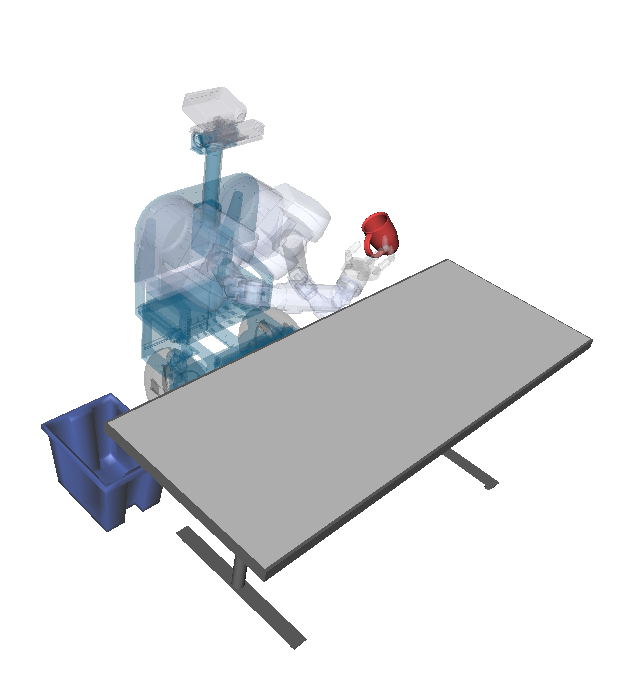
\includegraphics[width=2.7cm]{figs/herbarmmultithread/herbarmmultithread-step1.png}%
   \;
   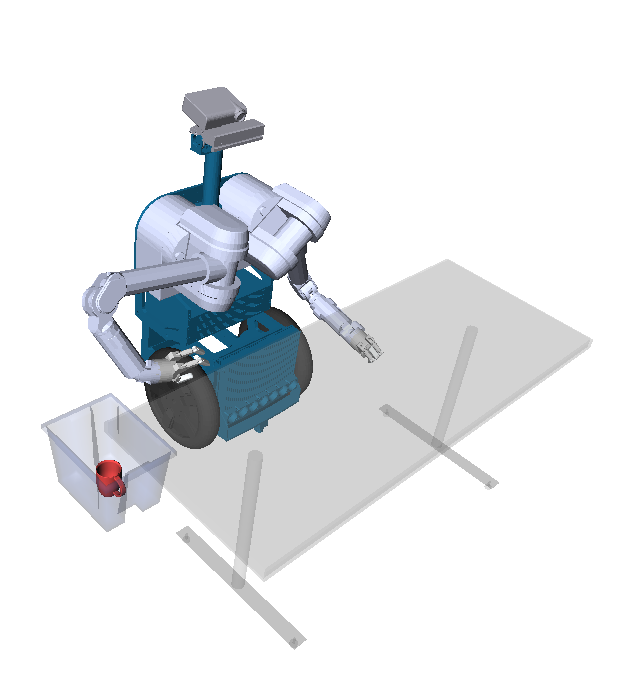
\includegraphics[width=2.7cm]{figs/herbarmmultithread/herbarmmultithread-step2.png}%
   
   \includegraphics{build/herbarmmultithread/master-fig}
   \caption[]{
      Results from a motion planning experiment for manipulation
      planning in which the robot must move to grasp the mug
      and place it into a bin at its side
      before returning to its initial configuration.
      In the course of planning the first step to the grasp point,
      the planner has discovered a number of edges known to be
      valid.
      After the grasp, the robot must find a motion to transfer the
      mug -- any edges known to be valid in the previous step
      can be used after only checking that the grasped mug does not
      collide with the environment.
      Compared with a sequence of single-query calls to LEMUR
      with model $\mathcal{C}_{\ms{simple}}$
      \protect\tikz{\protect\node[fill=black!80,draw=black]{};},
      LEMUR armed with the $\mathcal{M}_{\ms{family}}$ ensemble
      cost model
      \protect\tikz{\protect\node[fill=cyan,draw=black]{};}
      can guide the planner to use edges that are less
      expensive to validate.}
   \label{fig:family:herbarmmultithread-master}
\end{figure}

Here's some notes on the workcell example:

\begin{verbatim}
workcell basic (independent) atoms:
 (1) (robot) x (self+staticenv)
 (2) (robot) x (sheetstart)
 (3) (robot) x (sheetregrasp)
 (4) (robot) x (sheetend)
 (5) (robotgrabtop-sheetmidside2flat) x (self+staticenv)
 (6) (robotgrabtop-sheetside1flat) x (self+staticenv)
 (7) (robotgrabtop-sheetside1bent) x (self+staticenv)
 (8) (robotgrabbottom-sheetmidside1bent) x (self+staticenv)
 (9) (robotgrabbottom-sheetside2flat) x (self+staticenv)
(10) (robotgrabbottom-sheetside2bent) x (self+staticenv)

each problem step is built of atoms:
 step AB = (1) n (2)
 step BC = (1) n (5) n (6)
 step CD = (1) n (5) n (6)
 step EF = (1) n (5) n (7)
 step FG = (1) n (3)
 step GH = (1) n (8) n (9)
 step IJ = (1) n (8) n (10)
 step JA = (1) n (4)

FamilyUtilityChecker reports 17 vars (makes sense)

2**10 =  1024 truth table rows
\end{verbatim}

\section{Application: Exploiting Conservative Geometric Approximations}
\label{subsec:family:broad-phase}

The family formulation also enables motion planners to
reason directly about different robot or environment models.
For example, consider two geometric robot models,
one with high quality (e.g. from a CAD program),
and one hand-tuned ``padded'' model consisting of 
a small number of simple conservative bounding volumes.
The $\mathcal{C}$-subsets derived from these models
are related by $R_{\ms{padded}} \subseteq R_{\ms{CAD}}$.
Collision checkers currently use a similar approach internally
to speed up collision checks (see Fig.~\ref{fig:family:broad-phase}.
and Fig~\ref{fig:family:broad-phase-2d}).

See Figure~\ref{fig:family:broad-phase-2d}
for a simple example with integrated broad-phase collision checking
as described in Section~\ref{subsec:family:broad-phase}.

\begin{figure*}[b]
   \centering
   
   \subfloat[
      A single-set planner testing simply for membership in
      $\mathcal{C}_{\mbox{\scriptsize free}}$
      treats a collision validity checker as a
      ``black box.''
      Internally,
      modern checkers first employ an inexpensive broad-phase check
      using a low-dimensional conservative representation
      to quickly identify non-colliding bodies before
      resorting to an expensive narrow-phase check.
   ]{%
      \includegraphics{build/broadphase-single}%
   }%
   \quad%
   \subfloat[
      A family planner can explicitly reason about the
      conservative nature of the broad-phase check.
      This allows it to defer some narrow phase checks
      (often indefinitely)
      and instead prefer paths that require fewer expensive checks.
   ]{%
      \includegraphics{build/broadphase-multi}%
   }
   
   \caption[][0.0in]{Collision validity checking is a commonly used
     indicator function.
     The family formulation allows an intelligent planner to
     reach inside the checker's ``black box'' and reduce the number
     of costly narrow-phase checks.
     Resulting paths tend to be cheaper to compute and
     stay further from obstacles.}
   \label{fig:family:broad-phase}
\end{figure*}

% this is the broad phase bean figure
\begin{figure}
   \centering

   % left side
   \subfloat[Paths with lambda=0][%
      \centering
      Paths with $\lambda = 0$\par
      Average length: 733.0\par
      Average check cost: 7219.5
   ]{
      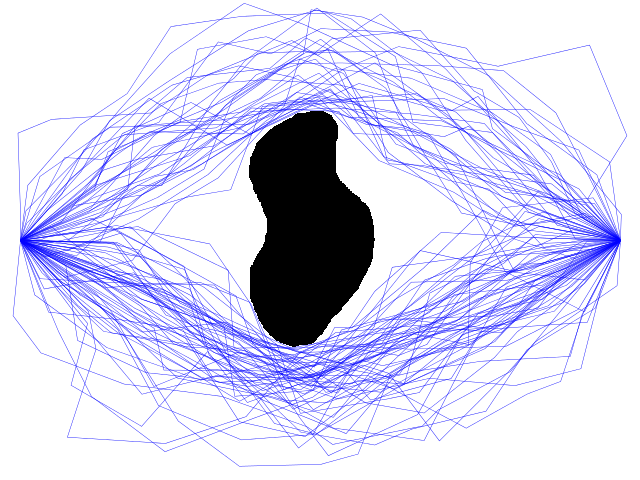
\includegraphics[width=0.45\textwidth]
      {figs/bean-allpaths-lambda0.png}
   }
   % right side
   \subfloat[Paths with lambda=1][%
      \centering
      Paths with $\lambda = 1$\par
      Average length: 836.5\par
      Average check cost: 4692.6
   ]{
      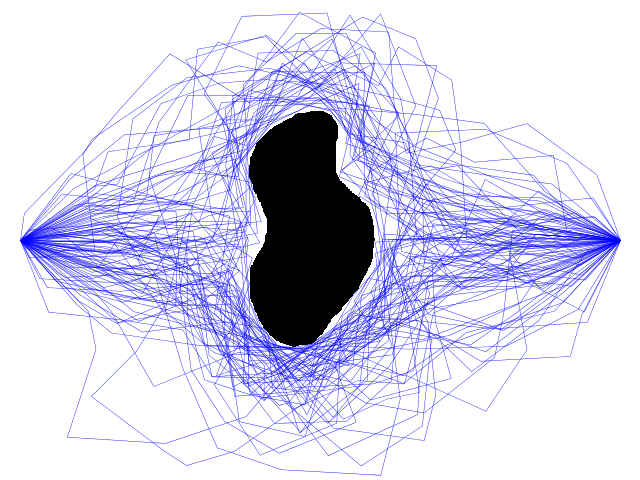
\includegraphics[width=0.45\textwidth]
      {figs/bean-allpaths-lambda1.png}
   }
   \\
   \subfloat[Paths with lambda=0][%
      \centering
      Paths with $\lambda = 0$\par
      Average length: 733.0\par
      Average check cost: 2685.7
   ]{
      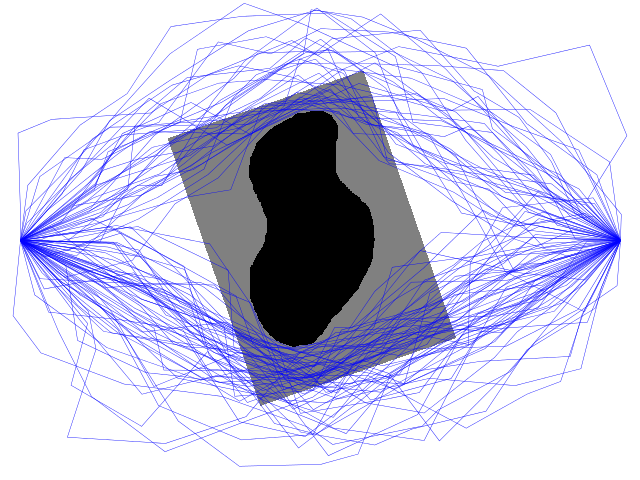
\includegraphics[width=0.45\textwidth]
      {figs/bean-allpaths-padded-lambda0.png}
   }
   % right side
   \subfloat[Paths with lambda=1][%
      \centering
      Paths with $\lambda = 1$\par
      Average length: 907.1\par
      Average check cost: 1064.5
   ]{
      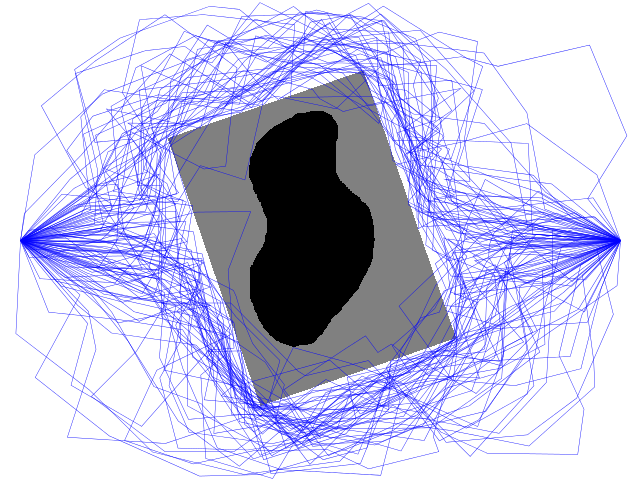
\includegraphics[width=0.45\textwidth]
      {figs/bean-allpaths-padded-lambda1.png}
   }

   \caption{A simple 2D example of the Family PRM using
     a broad-phase check.
     Checking for collision with the grey box is 10x less expensive
     than with the actual black obstacle.}
     %\cdnote{I need to talk about this in the text.}}
   \label{fig:family:broad-phase-2d}
\end{figure}

\section{Application: Dynamic Environments}

\paragraph{Dynamic Environments.}
\label{subsec:family:dynamic-environments}

\begin{figure}
   \centering

   \begin{minipage}{.6\textwidth}
      \begin{tikzpicture}
      \tikzset{>=latex} % arrow heads
      \node[anchor=south west,inner sep=0] at (0,0)
        {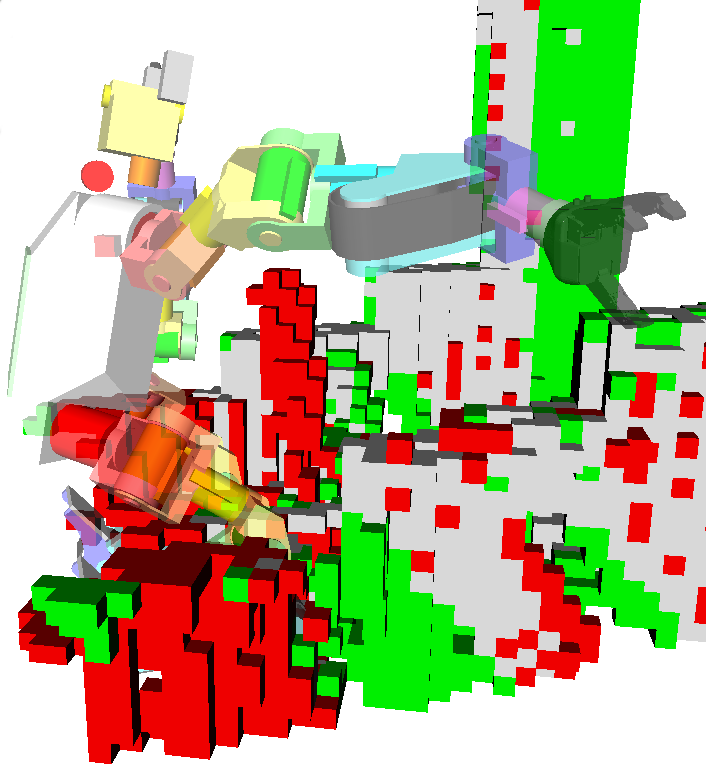
\includegraphics[width=0.8\textwidth]{figs/chimp-voxels-delta.png}};

      \node[draw,inner sep=3pt,fill=white,fill opacity=0.9,align=center]
        (debrislab) at (0.7,1.0) {Debris object\\removed};
      \node[circle,inner sep=2,draw,fill=white] (debris) at (2.2,2.9) {};
      \draw[draw=black, double=white, double distance=1pt, line width=1pt]
        (debrislab.north) -- (debris);
        
      \node[draw,inner sep=3pt,fill=white,fill opacity=0.9,align=center]
        (addlab) at (5.0,2.0) {Additional\\voxels seen};
      \node[circle,inner sep=2,draw,fill=white] (added) at (4.4,5.0) {};
      \draw[draw=black, double=white, double distance=1pt, line width=1pt]
        (addlab.north) -- (added);
        
      \end{tikzpicture}
   \end{minipage}%
   \,%
   \begin{minipage}{.35 \textwidth}
      \includegraphics{build/retroactive-a}
      
      \includegraphics{build/retroactive-b}
   \end{minipage}

   \caption{
      Structured or unstructured dynamic environments
      can be represented as a family problem
      (see Section~\ref{subsec:family:dynamic-environments}).
      
      \vspace{0.05in}
      \noindent
      (Left) A disaster response robot maintains a
      dynamic unstructured environment model
      using coarse voxels
      (scene data from a debris-clearing task at a
      recent disaster response competition).
      Since the last planning query,
      voxels have been added (green) and removed (red).
      
      \vspace{0.05in}
      \noindent
      (Right) $\mathcal{C}$-subsets and relations
      can be added retroactively.
      Here, the graph for an initial query is checked w.r.t $S_1$.
      After environment changes,
      $S_1$ is redefined in terms of the $\mathcal{C}$-subsets
      derived from the set of common, added, and removed elements,
      allowing for reuse on a query in $S_2$.
      Here,
      the planner need only check existing path segments
      against added voxels in order to reuse them for the current query.}
   \label{fig:family:dynamic-environments}
\end{figure}

The sensors on most articulated robots allow them to maintain
dynamic environment models to track changing collision geometry.
These models might be
structured (e.g. recognizing objects with known models)
or unstructured (e.g. occupancy models).
In both cases,
even in a changing world,
there are often areas that are fixed between planning queries.

Prior work (e.g. \citep{jaillet2004dynamicprm})
leverages this by imposing a dichotomy between
\emph{fixed} and \emph{moving} components of $\mathcal{C}$.
Our formulation extends this to an arbitrary number of such labels,
including ones defined retroactively (i.e. during planning;
see Fig.~\ref{fig:family:dynamic-environments}).
By explicitly labeling such areas in workspace
(and leveraging the \emph{set containment} property
\citep{newmanbranicky1991cspacetransforms}),
we can represent this structure as a family planning problem.

%\cdnote{%
%Special case of this is if objects are disappearing.
%Relation to occupancy grid representations of workspace
%(for deltas, conservative approxs, etc).}

% OTHER POTENTIAL APPLICATIONS:
%
%\subsubsection*{Conservative Bounding Volumes for Different Grasps}
%
%\subsubsection*{Conservative Bounding Volumes for Hypothesized Objects}
%
%There's a sweet ICRA paper here.
%
%\subsubsection*{Dual Arm Stuff}
%
%I think this is related.
%
%Check right arm against gian left side box, etc.
%
%\subsubsection*{Dimensionality Reduction}
%
%The Handey \cite{lozanoperez1987handey} robot
%assumed a box that contained the wrist links at a range of DOF values.
%
%\subsubsection*{Dual-Arm Stuff}
%
%This is very similar to dimensionality reduction.
%
%Loose coupling between arms.
%
%Separate roadmaps for each arm.
%
%Investigate this family structure.
